\documentclass[review]{elsarticle}


\usepackage{lineno,hyperref}
\newtheorem{definition}{Definition}
\usepackage{amssymb,amsmath,array}
\usepackage{xcolor}% provides \colorlet
\usepackage{fixme}
\usepackage{subfig}
\usepackage{float}
\fxsetup{
    status=draft,
    author=,
    layout=inline,
    theme=color
}

\definecolor{fxnote}{rgb}{0.8000,0.0000,0.0000}
% define the background colour:
\colorlet{fxnotebg}{yellow}

% refedine the layout macro:
\makeatletter
\renewcommand*\FXLayoutInline[3]{%
  \@fxdocolon {#3}{%
    \@fxuseface {inline}%
    \colorbox{fx#1bg}{\color {fx#1}\ignorespaces #3\@fxcolon #2}}}
\makeatother

\modulolinenumbers[5]

\journal{Journal of \LaTeX\ Templates}

\newcommand{\IR}{\rm \mathbb{R}}

%%%%%%%%%%%%%%%%%%%%%%%
%% Elsevier bibliography styles
%%%%%%%%%%%%%%%%%%%%%%%
%% To change the style, put a % in front of the second line of the current style and
%% remove the % from the second line of the style you would like to use.
%%%%%%%%%%%%%%%%%%%%%%%

%% Numbered
%\bibliographystyle{model1-num-names}

%% Numbered without titles
%\bibliographystyle{model1a-num-names}

%% Harvard
%\bibliographystyle{model2-names.bst}\biboptions{authoryear}

%% Vancouver numbered
%\usepackage{numcompress}\bibliographystyle{model3-num-names}

%% Vancouver name/year
%\usepackage{numcompress}\bibliographystyle{model4-names}\biboptions{authoryear}

%% APA style
%\bibliographystyle{model5-names}\biboptions{authoryear}

%% AMA style
%\usepackage{numcompress}\bibliographystyle{model6-num-names}

%% `Elsevier LaTeX' style
\bibliographystyle{elsarticle-num}
%%%%%%%%%%%%%%%%%%%%%%%

\begin{document}

\begin{frontmatter}

\title{The Conjunctive Disjunctive Graph Node Kernel for Disease Gene Prioritization}
%\tnotetext[mytitlenote]{Fully documented templates are available in the elsarticle package on \href{http://www.ctan.org/tex-archive/macros/latex/contrib/elsarticle}{CTAN}.}

%% Group authors per affiliation:
\author{Dinh Tran Van}
\author{Alessandro Sperduti}
\address{Department of Mathematics, Padova University, Trieste, 63, 35121 Padova, Italy}
\author{Fabrizio Costa}
\address{Department of Computer Science, University of Exeter Exeter EX4 4QF, UK}
%\fntext[myfootnote]{Since 1880.}

%% or include affiliations in footnotes:
%\author[mymainaddress,mysecondaryaddress]{Elsevier Inc}
%\ead[url]{www.elsevier.com}

%\author[mysecondaryaddress]{Global Customer Service\corref{mycorrespondingauthor}}
%\cortext[mycorrespondingauthor]{Corresponding author}
%\ead{support@elsevier.com}

%\address[mymainaddress]{1600 John F Kennedy Boulevard, Philadelphia}
%\address[mysecondaryaddress]{360 Park Avenue South, New York}

\begin{abstract}
Biological relations encoded in data sources are naturally represented in the form of graphs. As a consequence, a high number of graph-based biological learning systems have been proposed and shown promising results. In graph-based learning systems, one of the key points which determines their performance is the definition of the graph node similarity measure. Node similarities are normally measured by graph node kernels. However, most available graph node kernels do not show high discriminative capacity since they share two common limitations. First, they are based on the diffusion phenomenon which does not effectively exploit the nodes' context. Second, they are not able to process the auxiliary information associated to graph nodes.

In this paper, we propose an efficient graph node kernel that not only is able to effectively take into account nodes' context, but also to  exploit additional information  available on graph nodes. Empirical evaluation on disease gene prioritization shows that our proposed graph node kernel is able to reach  state-of-the-art performances when considering graph node kernels.

%Gene-disease associations are inferred on the basis of similarities between the proteins encoded by genes. Biological relationships used to define similarities range from interacting proteins, proteins that participate in pathways and protein expression profiles. Though graph kernel methods have become a prominent approach for association prediction, most solutions are based on a notion of information diffusion that does not capture the specificity of different network parts. Here we propose a graph kernel method that explicitly models the configuration of each gene's context. An empirical evaluation on several biological databases shows that our proposal achieves state-of-the-art results.
\end{abstract}

\begin{keyword}
Graph node kernels, graph decomposition, disease gene prioritization
\end{keyword}
\end{frontmatter}

\linenumbers
\section{Introduction}
The release of advanced technologies is one of the main reasons for the
revolution in various scientific research fields. In Biological and Medical
domains, modern technologies are making it not only easier but also more
economical than ever to undertake experiments and creating applications.
As a consequence, a vast amount of biological data in terms of volume
and type is generated through scientific experiments, published literature,
high-throughput experiment technology, and computational analysis. 
%% DINH!!!!! EARLIER VERSION OF THE SENTENCE BELOW WAS BASICALLY COPIED FROM: The European Bioinformatics Institute in 2016: Data growth and integration
This huge quantity of data is made available in the form of biological databases, accessible via different 
tools, such as web browsers, application programming interfaces, and scalable search
engines.
 
%% DINH!!!!! EARLIER VERSION OF THE SENTENCE BELOW WAS BASICALLY COPIED FROM: OMICs Technologies: Tools for Food Science
The nature of the data contained in biological databases concerns information about genes, such as their function, structure, and localization, as well as information about clinical effects of mutations and similarities of biological sequences and structures.

In the Biomedical field, disease-gene association recovery is a major goal that has received much attention from many researchers. Despite the fact that a big progress has been made in the last decades, the typical number of genes known to be related to a genetic disease is normally limited. In order to find out the remaining unknown set of genes related to the disease, one way is to search for them  in the whole genome or in specific regions that often contain a large number of suspected genes (candidate genes). This is obviously not a good approach since it is expensive, not only in terms of time consumption, but also from a financial point of view. For this reason, many gene prioritization methods, which automatically predict a list of candidate genes sorted according to the probability to be actually involved in the target disease, have been proposed in literature. Predictive systems for gene-disease association are often based on a notion of similarity between genes inferred from the available knowledge encoded in the biological databases. In addition, many of them exploit machine learning methods to predict the gene-disease associations. Moreover, a common strategy is to encode relations between genes as a network where two genes are connected each other if they turn out to be very similar. Graph based techniques are then used to make useful inferences, as in \cite{mordelet2011prodige, chen2014disease,valentini2014extensive}.

One of the key points that determines the performance of graph-based biological learning systems in general, and graph-based gene-disease  prioritization systems in particular, is the definition of the node similarity measure. The node similarity is often measured by graph node kernels \cite{kondor2002diffusion,chen2014disease,fouss2006experimental,chebotarev2006matrix}. The state-of-the-art graph node kernels used to measure node similarity are based on the notion of information diffusion, which mainly depends on the number of paths connecting two nodes in the graph. These graph node kernels often show relatively low discriminative capacity, especially when working with sparse graphs (i.e., graphs with a  low number of  links), because of the following limitations. First, they are defined using a heat diffusion dynamics which sums up the contributions of all  paths from one node to another one, disregarding the local topological context of the nodes and considering the single contribution of one path as independent with respect to the contributions of other paths.
Second, they do not take into account additional information (i.e. properties of a single node) eventually associated to nodes of graphs, when available. These additional information normally provide a complement to the graph topology, and as such may contribute to improve, if used, the expressiveness of the kernel. 

In this paper, we propose an effective convolutional graph node kernel, named \textit{Conjunctive Disjunctive Node Kernel} (CDNK) which is able to: \textit{i}) effectively exploit the nodes' context; \textit{ii}) involve in the computation of the kernel the additional information attached to graph' nodes, when available.
In particular, in CDNK, first, the graph is transformed into a set of linked
connected components in which we distinguish between “conjunctive” links
whose endpoints are in the same connected components and “disjunctive”
links that connect nodes located in different connected components. Then
the similarity between any couple of nodes is measured by employing a
particular graph kernel on two neighborhood subgraphs rooted at each
node. Next, it integrates the side information by applying convolution
of the discrete information with the real valued vectors associated to
graph nodes. 

\section{Background}
In this section, we first introduce definitions and notations that are used to define our proposed method. We then describe the state-of-the-art concerning graph node kernels.
\subsection{Definitions and Notations}
A graph is a structure $G=(\mathbb{V},\mathbb{E}, \mathcal{L}_1, \mathcal{L}_2)$ where $\mathbb{V}$, $\mathbb{E}, \mathcal{L}_1, \mathcal{L}_2$ are the vertex (node) set, link (edge) set, discrete labeling fuction and real vector labeling function, respectively. The functions $\mathcal{L}_1, \mathcal{L}_2$ are defined as:
\begin{itemize}
\item $\mathcal{L}_1: \mathbb{V} \longmapsto \mathbb{L}$, where $\mathbb{L}$ is a set of discrete labels. $\mathcal{L}_1$ assigns a single discrete label $\ell \in \mathbb{L}$ for each node $v \in \mathbb{V}$, $\mathcal{L}_1(v) = \ell$. 
\item $\mathcal{L}_2: \mathbb{V} \longmapsto \mathbb{R}^n$. $\mathcal{L}_2$ assigns a single real vector label $(v_1,v_2,\ldots,v_n) \in \mathbb{R}^n$ for each ndoe $v \in \mathbb{V}$, $\mathcal{L}_2(v) = (v_1,v_2,\ldots,v_n)$.
\end{itemize}

We define the length of a shortest path between $u$ and $v$, denoted as $\mathcal{D}(u,v)$, as the number of edges on a shortest path between them. The \textit{neighborhood} of a node $u$ with radius $r$, $N_r(u) = \lbrace v\ |\ \mathcal{D}(u,v) \leq r \rbrace$, is the set of nodes at distance no greater than $r$ from $u$. The corresponding \textit{neighborhood subgraph} $\mathcal{N}_{r}^{u}$ is the  subgraph induced by the neighborhood (i.e. considering all the edges with endpoints in $N_r(u)$). The \textit{degree} of a node $u$, $deg(u) = |\mathcal{N}_{1}^{u}|$, is the cardinality of its neighborhood for $r=1$. The maximum node degree in the graph $G$ is $deg(G)=\max_{v\in \mathbb{V}}deg(v)$.

\begin{definition}{}
\textit{An adjacency matrix $\textbf{A}$ is a symmetric matrix used to characterize the direct links between vertices $v_{i}$ and $v_{j}$ in the graph. Any entry $A_{ij}$ is equal to $w_{ij}\in \mathbb{R}$ when there exists a link connecting $v_{i}$ and $v_{j}$, and is 0 otherwise.}. 
\end{definition}

\begin{definition}{}
\textit{The Laplacian matrix $\textbf{L}$ is defined as $\textbf{L} = \textbf{D}-\textbf{A}$, where $\textbf{D}$ is the diagonal matrix with non-null entries equal to the summation over the corresponding row of the adjacency matrix, i.e. $\textbf{D}_{ii}=\sum_j \textbf{A}_{ij}$.}
\end{definition}

\begin{definition}{}
\textit{The Transition matrix of a graph $G$, denoted as $\textbf{P}$, is a matrix with entries $P_{ij} = A_{ij}/\sum_{i}^{}A_{ij}$. When considering a random walk in $G$, $P_{ij}$ can be interpreted as proportional to the probability of moving from node $v_i$ to  node $v_j$.}
\end{definition}

\subsection{Kernels on Graphs}
Kernel methods have emerged as one of the most powerful framework in machine learning. They have been successfully applied in various domains, due to their modularity, i.e. the definition of kernel functions is independent from the design of the learning algorithm. 

A kernel function can be  considered as the similarity measure between input instances, whatever the nature of the instances may be, e.g. vectors, sequences, trees, graphs.
% in the feature space. Interestingly, It can be defined in feature space and with any type of data representation. 
Formally, a kernel $k: \mathbb{X} \times \mathbb{X}\longmapsto \mathbb{R}$, where $\mathbb{X}$ is a set of entities, is a function satisfying the following properties: \textit{i}) $k$ is symmetric, i.e., $k(x_1,x_2) = k(x_2,x_1)$, where $x_1, x_2 \in \mathbb{X}$; \textit{ii}) $k$ is positive semi-definite, that is $\sum_{i=1}^{N}\sum_{j=1}^{N} c_i c_jk(x_i,x_j) \geq 0$ for any $N>0$, $c_i, c_j \in \mathbb{R}$, and  $x_i, x_j \in \mathbb{X}$. 

Canonical machine learning methods take vectorial data, i.e. numerical vectors that collect the results of measures on features of the input instances, as their input. However, there are many fields where data is naturally represented by structured forms, such as graphs, one of the most popular representations for structured data. 
Two interesting examples of domains involving graphs are Chemistry and the Web. In Chemistry, chemical compounds are represented via their molecular graphs and typical computational tasks consist in the prediction of their physicochemical properties. Thus, in this domain, the target function to learn is a mapping from one graph to a real value. The Web can be described as a huge graph, where nodes are web pages and edges are links from one page to another one.  A typical task in this context is to automatically predict the topics covered by the textual content of a page on the basis of the characteristics of web pages connected with it. So, the  target function to learn is a mapping from one node of the graph to a set of discrete values.
Therefore, the definition of a kernel function for graphs has to take into account one of the two scenarios described above.
In the first case, we talk about graph kernels, while in the second case we talk about graph node kernels. Both graph kernels and graph node kernels are widely applied to build graph-based learning systems for fields ranging from Social Sciences, to Recommendation Systems, and Biology. 

In general, one important contribution with respect to the design of kernels for structured data, and in particular for graphs, has been given by Haussler, who proposed a convolution-based framework for the definition of decompositional kernels \cite{haussler1999convolution}. 
In the following, we shortly describe some of the state-of-the-art graph (node) kernels underpinning our proposed approach.

%Examples are kernels proposed in \cite{shervashidze2011weisfeiler, gartner2003survey, borgwardt2005shortest, costa2010fast}. Following we describe NSPDK \cite{costa2010fast}, a convolutional graph kernel which shows state of performance and it is later on used to define our proposed graph node kernel.
\subsubsection{Graph Kernels}
\label{graph-kernels}
The task of designing efficient and expressive graph kernels plays an important role in the development of graph-based predictive systems. Existing graph kernels are decompositional kernels and can be classified into two categories: sequence-based graph kernels and subgraph-based graph kernels. The sequence-based graph kernels decompose graphs into ``parts" in sequence-based forms, such as paths and walks. Typical examples of sequence-based graph kernels are the product graph kernel \cite{gartner2003survey}, and the shortest path kernel \cite{borgwardt2005shortest}. The subgraph-based graph kernels decompose graphs into subgraphs. Examples include the Weisfeiler-Lehman kernel \cite{shervashidze2009fast, shervashidze2011weisfeiler}, and the Neighborhood Subgraph Pairwise Distance Kernel (NSPDK) \cite{costa2010fast}. 
This latter category of kernels are generally more effective because sub-graphs are more expressive than walks and paths.
Moreover, they can be computed quite efficiently thanks to sparsity of representation that allows an explicit encoding of the graph via hash functions.
In the following, we describe NSPDK, since it is later adopted to develop the proposed graph node kernel (presented in Section \ref{method}).

The NSPDK \cite{costa2010fast} is an instance of convolution kernel \cite{haussler1999convolution} where a given
 graph $G$ is decomposed in features (pairwise neighborhood subgraphs) constituted by couples of subgraphs of radius $r$ rooted at nodes of $G$ which are
 at distance $d$. More formally, given two rooted graphs $A_u, B_v$, where $u$ and $v$ are nodes of $G$, the relation $R_{r,d}(A_u, B_v, G)$ is true {\em iff}  $\mathcal{D}(u,v)= d$ and $A_u \cong \mathcal{N}_r^u$ is (up to isomorphism $\cong$) a neighborhood subgraph of radius $r$ of $G$ as well as $B_v \cong  \mathcal{N}_r^v$. Figure \ref{fig:nspdk} illustrates a pairwise neighborhood subgraph. We denote with $R^{-1}$ the inverse relation that returns all pairs of neighborhoods of radius $r$ at distance $d$ in $G$, $R^{-1}_{r,d}(G) = \lbrace (A_u, B_v) | R_{r,d}(A_u,B_v,G)=true\rbrace$. The kernel $\kappa_{r,d}$ over $\mathcal{G} \times \mathcal{G}$, counts the number of such fragments in common in two input graphs: 
\begin{center}
$\kappa_{r,d}(G,G^{'}) = 
\!\!\!\!\!\!\!\!\!\!\!\! 
\sum\limits_{\substack{(A_u, B_v) \ \in \ R_{r,d}^{-1}(G) \\ 
({A'}_{u^\prime}, {B'}_{v'}) \ \in \ R_{r,d}^{-1}(G')
}} \!\!\!\!\!\!\!\!\!\!\!\!  { { \textbf{1}_{A_{u} \cong A'_{u^\prime}}} \cdot {
\textbf{1}_{B_{v} \cong B'_{v'}}} }$, 
\end{center} 
\noindent where $\textbf{1}_{A \cong B}$ is the \textit{exact matching function} that returns 1 if $A$ is
isomorphic to $B$ and 0 otherwise.  Finally, the NSPDK is defined as $K(G,G') = \sum\limits_{r}{\sum\limits_{d}{\kappa_{r,d}(G,G')}}$, where for efficiency reasons, the values of $r$ and $d$ are upper bounded by  given maximal values $r^*$ and $d^*$, respectively.
\begin{figure}
\centering
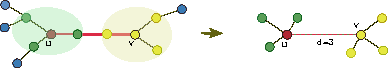
\includegraphics[width=.9\textwidth]{nspdk}
\caption{\label{fig:nspdk} Example of pairwise neighborhood subgraphs for nodes $u$ and $v$ with $r=1$ and \mbox{$d=3$}. {\it Left:} input graph where the nodes $u$ and $v$ are connected by a shortest path (highlighted in red) of length 3; the neighborhood subgraphs of radius $1$ rooted at $u$ (highlighted in green) and at $v$ (highlighted in yellow) are shown as well. {\it Right:} representation of the induced pairwise neighborhood subgraphs feature.}
\end{figure}

\subsubsection{Graph Node Kernels}
The state-of-the-art diffusion-based kernels for nodes are based on the same equations used to model the heat diffusion phenomenon. In other words, they take paths connecting two nodes into account when measuring their similarity. In the following, we shortly introduce some of the most used diffusion-based graph node kernels.

%\begin{itemize}
%\item 
{\it Laplacian exponential diffusion kernel.} One of the most well-known graph node kernels is the Laplacian exponential diffusion kernel (DK), as it is widely used for exploiting discrete structures in general and graphs in particular. On the basis of the heat diffusion dynamics, Kondor and Lafferty proposed DK in \cite{kondor2002diffusion}: imagine to initialize each vertex with a given amount of heat and let it flow through the edges until an arbitrary instant of time. The similarity between any vertex couple $v_{i}$, $v_{j}$ is the amount of heat starting from $v_{i}$ and reaching $v_{j}$ within the given time. Therefore, DK can capture the long range relationship between vertices of a graph to define the global similarities. Below is the formula to compute LEDK values:
\begin{equation} 
\label{LEDK-formula}
\textbf{K} = e^{-\beta \textbf{L}} = \textbf{I} - \beta \textbf{L} + \frac{\beta \textbf{L}^{2}}{2!} - ...
\end{equation}
where $\beta$ is the diffusion parameter and is used to control the rate of diffusion, and $\textbf{I}$ is the identity matrix. Choosing a consistent value for $\beta$ is very important: on the one side, if $\beta$ is too small, the local information cannot be diffused effectively and, on the other side, if it is too large, the local information will be lost. DK is positive semi-definite as proved in \cite{kondor2002diffusion}.

%\item 
{\it Exponential diffusion kernel.} In DK, the similarity values between high degree vertices are generally higher compared to those between low degree ones. Intuitively, the more paths connect two vertices, the more heat can flow between them. This could be problematic since peripheral nodes (i.e., low degree nodes) have unbalanced similarities with respect to central nodes (i.e., high degree nodes). In order to make the strength of individual vertices comparable, a modified version of DK is introduced by Chen et al in \cite{chen2014disease}, called Markov exponential diffusion kernel (MED) and given by the following formula:
\begin{equation} \label{MEDK-formula}
\textbf{K} = e^{-\beta \textbf{M}}.
\end{equation}
The difference with respect to the Laplacian diffusion kernel is the replacement of $\textbf{L}$ by the matrix $\textbf{M}=(\textbf{D}-\textbf{A}-n\textbf{I})/n$ where $n$ is the total number of vertices in the graph. In particular, the introduced modification of the Laplacian is designed to compensate the problem described above via a sort of normalization of the degree of vertices. The role of $\beta$ is the same as for DK.

%\item 
{\it Markov diffusion kernel.} The original Markov diffusion kernel (MD) was introduced by Fouss et al. \cite{fouss2006experimental} and exploits the idea of diffusion distance, which is a measure of how similar the pattern of heat diffusion  between a pair of  nodes is. In other words, it expresses how much nodes ``influence'' each other in a similar fashion. If their diffusion patterns are alike, the similarity will be high and, vice versa, it will be low if they diffuse differently. This kernel is computed as:
\begin{equation} 
\label{MDK-formula}
\textbf{K} = \textbf{Z}(t)\textbf{Z}^{\top}(t),
\end{equation}
where $\textbf{Z}(t) = \frac{1}{t}\sum_{\tau=1}^{t}\textbf{P}^{\tau}$, and $\textbf{P}$ is the transition matrix.

%\item 
{\it Regularized Laplacian kernel.} Another popular graph node kernel function used in graph mining is the regularized Laplacian kernel (RL). This kernel function was introduced by Chebotarev and Shamis in \cite{chebotarev2006matrix}, and it implements a normalized version of the random walk with restart model. It is defined as follows:
\begin{equation} 
\label{RLK-formula}
\textbf{K} = \sum_{n=0}^{\infty}\beta^{n}(-\textbf{L})^n = (\textbf{I} + \beta \textbf{L})^{-1},
\end{equation}
where the parameter $\beta$ is again the diffusion parameter. RL counts the paths connecting two nodes on the graph induced by taking $-\textbf{L}$ as the adjacency matrix, regardless of the path length. Thus, a non-zero value is assigned to any couple of nodes as long as they are connected by any indirect path. RL remains a relatedness measure even when the diffusion factor is large, by virtue of the negative weights assigned to self-loops.

%\end{itemize}
\section{A New Graph Node Kernel}
\label{method}
As already argued in the introduction, diffusion-based kernels compute the similarity between two nodes only on the basis of how well they are connected within the graph. Thus, it can be stated that they exploit the global topology of the graph to compute the output. Small values of the diffusion parameter $\beta$ can be used to give more emphasis to shorter paths with respect to longer ones in order to take into account the local topology around a node, however the effect of this setting is homogeneous through the whole set of nodes. 
The kernel we propose in this paper is, on the contrary, based on the exploitation of a more detailed information on the local topology around a node. We obtain this information by using, in a specific way, the similarity notion computed by the neighborhood based decomposition kernel NSPDK \cite{costa2010fast}. The underpinning idea of the new kernel is to capture local topological information by looking at local  subgraphs rooted at the two nodes of interest. This can be done, in principle, by a direct application of the NSPDK kernel to the local subgraphs. In practice, when a node has a high degree, the local subgraph may be quite large and, since NSPDK is based on exact matching, the probability to have an exact match between the two local subgraphs decreases with the increase of  node degree. For this reason, we propose to decompose the original graph into a set of sparse connected components that singularly have lower node degree with respect to the original graph. The above idea is then applied to these set of components, and the novel kernel is computed by summing up all the obtained contributions from these components.  
In addition to that, we also extend the definition of the kernel in such a way to allow  the involvment  of additional information, that may be associated to each node, in the computation. In the following, we give a more detailed description of the proposed kernel.

Given an input undirected labeled graph $G=(\mathbb{V},\mathbb{E}, \mathcal{L}_1, \mathcal{L}_2)$, the computation of our kernel consists of two phases. In the first phase, a network decomposition procedure is applied to transform the graph into a set of linked sparse connected components. In this procedure, we define two different kinds of link: \textit{conjunctive} and \textit{disjunctive}, that we treat in distinct manners.
Nodes linked by conjunctive edges are going to be used jointly to define the notion of context and will be visible to the NSPDK neighborhood graph kernel. Nodes linked by disjunctive edges are instead used to define features based only on the pairwise co-occurrence of the genes at the endpoints and are processed by our novel kernel. In the second step, the similarity between any node couple ($u$, $v$) is computed by applying NSPDK to the two neighborhood subgraphs rooted at nodes $u$ and $v$, extracted from the graph obtained from the first decomposition phase. In the following, we describe each phase in detail.

\subsection{Network Decomposition} 
\label{network-decomposition}
In genetic networks, it is not uncommon to find nodes with high degrees. Unfortunately these cases cannot be effectively processed by a neighborhood based decomposition kernel (see Section \ref{graph-kernels}) since these are based on the notion of exact matches. Neighborhood subgraphs rooted at high degree nodes are relatively big due to a high number of neighbors and edges. Since the number of non-isomorphic graphs grows exponentially with the number of nodes and edges, this leads to a low likelihood of finding neighborhood subgraphs rooted at high degree nodes which are isomorphic. 
%Thus, the probability of having identical neighborhoods decreases exponentially as the degree increases.  
This means that in a finite network it quickly becomes impossible to find any match and hence to learn or to generalize at all. 

In order to solve the above problem, we propose a procedure to ``sparsify'' the input network. In practice, we mostly keep the same the cardinality of the edge set. However, we mark the edges with special attributes so that the novel kernel is able to treat them differently during computation. The result is a procedure that decomposes the network in a linked collection of sparse sub-networks where each node has a reduced connectivity when considering the edges of a specific type. However the other edges are still available to connect the various sub-networks. 

\textit{Iterative k-core decomposition} \cite{alvarez2005k}: the node set is partitioned in two groups on the basis of the degree of each node w.r.t. a threshold degree $D$, the first part contains all nodes with degree smaller than or equal to $D$ and the second part the remaining ones. The node partition is used to induce the ``conjunctive'' vs ``disjunctive'' notion for the edge partition: edges that have both endpoints in the same part are marked as conjunctive, otherwise they are marked as disjunctive. We apply the k-core decomposition iteratively, where at each iteration we consider only the graph induced by the conjunctive edges. We stop iterating the decomposition after a user defined number of steps. Note that this decomposition does not alter the cardinality of the edge set, it is simply a procedure to mark each edge with the attribute conjunctive or disjunctive.  

\begin{figure}
\centering
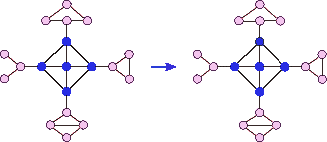
\includegraphics[width=.9\textwidth]{k_core}
\caption{Example of application of one step of \textit{k-core decomposition} using degree threshold $D = 3$. {\it Left:} the input graph. \textit{Right:} resulting marking of the edges: an edge $(u,v)$ is marked as {\it disjunctive} (represented by dashed line) if either $ deg(u) \leq 3 \wedge  deg(v) > 3 $ or $ deg(u) > 3 \wedge  deg(v) \leq 3 $; all remaining edges are marked as {\it conjunctive} (represented by solid line).}
\label{fig:kcore-decomposition}
\end{figure}

\textit{Clique decomposition} \cite{tarjan1985decomposition}: to model the notion that nodes in a clique are tightly related, we summarize the whole clique with a new ``representative'' node. All the cliques (completely connected subgraphs) with a number of nodes greater than or equal to a given threshold  $C$ are identified. The endpoints of all edges incident on the clique's nodes are moved to the representative node. Disjunctive edges are introduced to connect each node in the clique to the representative. Finally all edges with both endpoints in the clique are removed.

In our work a graph $G$ is transformed by  first applying the iterative k-core decomposition and then the clique decomposition. Let denote with $G^{\wedge\vee}$ the graph obtained as output of this transformation.

\begin{figure}
\centering
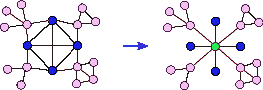
\includegraphics[width=.9\textwidth]{cliques.pdf}
\caption{Example of application of the {\it clique decomposition} step using threshold $C = 4$. {\it Left:} the input graph; nodes coloured in blue belong to a clique of size 4. \textit{Right:} the resulting graph after {\it clique decomposition}; a representative node (green color) is introduced for the clique of size 4; edges belonging to the clique are removed, while disjunctive edges are introduced to connect each node in the clique to the representative; in addition, edges not belonging to the clique but with one endpoint in clique's nodes  are moved  to the representative node. }
\label{fig:clique-decomposition}
\end{figure}

\subsection{The Conjunctive Disjunctive Node Kernel}
%We start from the Neighborhood Subgraph Pairwise Distance Kernel (NSPDK) \cite{costa2010fast} and adapt it to express the similarity between nodes in a single network. The key idea in NSPDK is to decompose graphs in small fragments and count how many pairs of fragments are shared between two instances. We introduce two improvements: \textit{i}) we partition the features according to the individual node's neighborhood, and \textit{ii}) we introduce a  distinction between ``disjunctive'' and ``conjunctive'' edges.

We define a node kernel $K(u,u^\prime)$ between  nodes $u$ and $u^\prime$ belonging to $G^{\wedge\vee}$ as follows.
% The idea is to define the features of a node $u$ as the subset of NSPDK features that always have the node $u$ as one of the roots.  THIS SENTENCE IS NOT TRUE!!
%In addition we distinguish between two types of edges, called {\em conjunctive} and {\em disjunctive} edges. THIS IS  A REPETITION
When computing distances to induce neighborhood subgraphs, only conjunctive edges are considered. When choosing the
pair of neighborhoods to form a single feature, we additionally consider roots $u$ and $v$ that are not at distance $d$ but such that $u$ is connected to $w$ via a disjunctive edge and such that $w$ is at distance $d$ from $v$ (Figure \ref{fig:cdnk} is an illustration). In this way disjunctive edges can still allow an {\em information flow} even if their
endpoints are only considered in a pairwise fashion and not jointly. 

In order to obtain a formal definition of the proposed kernel, we start by defining new specific notions of distance and neighborhood subgraph, which only depends on conjunctive edges. With $\mathcal{D}^{\wedge}(u,v)$ we denote the  length of a shortest path between $u$ and $v$ (belonging to $G^{\wedge\vee}$) where all edges are conjunctive edges. We can then define $N^{\wedge}_r(u) = \lbrace v\ |\ \mathcal{D}^{\wedge}(u,v) \leq r \rbrace$
and the {\it conjunctive neighborhood subgraph} $\mathcal{N}_{r}^{\wedge u}$ as the  subgraph induced by $N^{\wedge}_r(u)$ only considering conjunctive edges. We can now define 
two relations: the \textit{conjunctive relation} $R^{\wedge}_{r,d,u}(A_w, B_v, G^{\wedge\vee})$, which is true 
{\em iff}  $w = u$ and $\mathcal{D}^{\wedge}(w,v)= d$ and $A_w \cong \mathcal{N}_r^{\wedge w}$ is (up to isomorphism $\cong$) a conjunctive neighborhood subgraph of radius $r$ of $G^{\wedge\vee}$ as well as $B_v \cong  \mathcal{N}_r^{\wedge v}$;
the \textit{disjunctive relation} $R_{r,d,u}^{\vee}(A_w, B_v, G^{\wedge\vee})$ which is true {\em iff} $w = u$ and $A_w \cong \mathcal{N}_r^{\wedge w}$ and $B_v \cong \mathcal{N}_r^{\wedge v}$ are true and $\exists z$ s.t. $\mathcal{D}^{\wedge}(z,v)= d \wedge (w,z)$ is a disjunctive edge. 

We define $\kappa^{\wedge\vee}_{r,d}$ on the  inverse relations ${R^{\wedge -1}_{r,d,u}}$ and ${R^{\vee -1}_{r,d,u}}$:
\begin{center}
 $\kappa^{\wedge\vee}_{r,d}(u,u^\prime) = \!\!\!\!\!\!\!\!\!\!\!\!
 \sum\limits_{\substack {A_u,{B}_{v} \in {R_{r,d,u}^{\wedge -1}}(G^{\wedge\vee}) \\ A'_{u^\prime},{B'}_{v'} \in {R_{r,d,u^\prime}^{\wedge -1}}(G^{\wedge\vee}) }} \!\!\!\!\!\!\!\!\!\!\!\!
  { \textbf{1}_{A_u \cong A'_{u^\prime}} \cdot { \textbf{1}_{B_{v} \cong B'_{v'}}}}
+ \!\!\!\!\!\!\!\!\!\!\!\!
 \sum\limits_{\substack {A_u,{B}_{v} \in {R_{r,d,u}^{\vee -1}}(G^{\wedge\vee}) \\
  A'_{u^\prime},{B'}_{v'} \in \ {R_{r,d,u^\prime}^{\vee -1}}(G^{\wedge\vee}) }} \!\!\!\!\!\!\!\!\!\!\!\!
  { \textbf{1}_{A_u \cong A'_{u^\prime}} \cdot { \textbf{1}_{B_{v} \cong B'_{v'}}}}
  $.
\end{center}
The CDNK is finally defined as $K(u,u^\prime) = \sum\limits_{r}{\sum\limits_{d}{\kappa^{\wedge\vee}_{r,d}(u,u^\prime)}}$, where once again for efficiency reasons, the values of $r$ and $d$ are upper bounded to a given maximal $r^*$ and $d^*$.

\begin{figure}
\centering
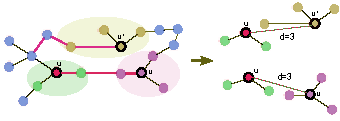
\includegraphics[width=.9\textwidth]{cdnk}
\caption{\label{fig:cdnk} Examples of two pairwise neighborhood subgraphs for the $u$ node with $r=1$ and $d=3$ using \textit{conjuctive} and \textit{disjuctive} edges. {\it Left:} input graph where nodes $v$ and $v^\prime$ have a {\it conjunctive} shortest path (highlighted in red) of length $3$ with $u$;  {\it conjunctive} neighborhood subgraphs of radius $1$ for $u$ (highlighted in green), $v$ (highlighted in violet), $v^\prime$ (highlighted in yellow)  are shown as well. {\it Right:} representation of the two induced pairwise \textit{conjuctive} neighborhood subgraphs.} 
\end{figure}

\subsection{Additional Node Information}
In order to integrate the information of real vector labels that may be present associated to nodes, we proceed as follows. We compute a sparse vector representation for the conjunctive neighborhood graph rooted at node $u$ following \cite{costa2010fast}: for each conjunctive neighborhood subgraph we calculate the quasi-isomorphism certificate hash code; we then combine the hashes for the pair of neighborhoods and use the resulting integer as a feature indicator. This yields a direct sparse vector representation (associated to node $u$ in graph $G^{\wedge\vee}$) $f: u \longmapsto \mathbb{R}^N$ where $N \approx 10^6$. Given the real valued vector information associated to nodes in graph $G^{\wedge\vee}$, we also cluster\footnote{Any clustering algorithm that returns cluster representations provided of a function to measure the similarity of a vector with respect to a given cluster will do the job.} them in $P$ clusters (c.f.r. Section \ref{sec:lab}) and define a function $g: u \longmapsto \mathbb{R}^P$ which returns the multi-class similarity w.r.t. each of the $P$ cluster (prototypes). 

A new version of CDNK considering the discrete convolution of the discrete information with the real valued information can now be computed as:   
\begin{equation}
K(u,u^\prime) = \left< f(u) \bigotimes g(u), f(u^\prime) \bigotimes g(u^\prime) \right>,
\end{equation}
where the discrete convolution is defined as: 
$(f \bigotimes g)[n]=\sum _{m=0}^{K-1}f[n-m]g[m])$.
In words, we place a scaled copy of the real valued vector at the position indicated by each feature computed on the basis of the discrete information. Intuitively, when both the real valued and the discrete information match, the kernel computes a large similarity, but if there is a discrepancy in either one of the sources of information, the similarity will be penalized. 

\subsection{Hyper-parameter Space}\label{hyper}
Our kernel consists of five hyper-parameters: the threshold degree $D$, the clique size threshold $C$, the maximal radius $r^*$, the maximal distance $d^*$, and the number of clusters $P$. In order to choose the optimal tuple of   values for kernel hyper-parameters in a specific setting, a model selection procedure is normally adopted. The hyper-parameter space of our kernel is potentially large due to the relatively high number of hyper-parameters. However, all hyper-parameters are integer variables and it makes sense to use only small values for them. For example, the value of the threshold degree $D$ should neither be too high nor too low: if it is high, the neighborhood subgraphs are going to be too big and the isomorphism check becomes inefficient; vice versa, if it is too low, the decomposed graph contains connected components which are too sparse to allow learning to be effective. Moreover, it is reasonable to keep the clique size threshold $C$ 
within a narrow range of values in order to avoid the removal of too many edges. Concerning the maximal radius $r^*$,  too  high values will lead again to big neighborhood subgraphs, especially in graphs with a high node degree average. The maximal distance $d^*$ can be set with small values since the average shortest distance length between nodes of biological networks is relatively low. Finally, if the value assigned to $P$ is too low, all nodes basically get the same information attached to them and thus the labels are not informative; vice versa, if a high value is used, there will be very few matches and the kernel will be extremely sparse, making learning ineffective.

%Our kernel consists of five parameters: the threshold degree $D$, clique size threshold $C$, maximal radius $r^*$, maximal distance $d^*$ and number of clusters $P$ clusters in which their values are in $\mathbb{N}^*$. In order to choose the optimal tuple of parameters for kernel in a specific setting, a model selection procedure is normally adopted from a determined subset of parameter space. The parameter space of our kernel seems large due to the relatively high number of parameters. However, most parameter values are supposed to be in limited ranges. Therefore, it is actually not too big. In particular, the clique size threshold $C$ is recommended to be in $\lbrace 4, 5\rbrace$. The maximal radius $r^*$ is set with a value smaller than or equal to $3$ since it will lead to big neighborhood subgraphs (as discussed in \ref{network-decomposition}). The maximal distance $d^*$ is assigned with values less than or equal to $4$ because the value of the maximal shortest distance between nodes in a connected component is often not too high. The values of the threshold degree $D$ should neither be too high and too low. If it is high, we have to face with high degree node problem, and if it is too low, the obtained graph consists of too sparse connected components. Therefore, we suggest the value for $D$ is in $\left[6, 20 \right]$. 

\section{Empirical Evaluation}
\label{empirical-evaluation-cdnk}
In this section, we evaluate the performance of CDNK versus other graph node kernels. Specifically, we focus on the following two questions:
\begin{itemize}
\item {\it Q1}: Does CDNK show better performance with respect to other graph node kernels?
\item {\it Q2}: Does the use of local topology (as envisioned in the proposed kernel) and/or additional information (real vector labels) help to  improve the performance of CDNK?
\end{itemize}

\subsection{Experimental Settings and Evaluation Methods}
We carry out experiments in the context of disease gene prioritization where the aim is to build a learning system which allows to prioritize candidate genes based on their probabilities of being associated to a given genetic disease.

The learning pipeline typically used for this kind of tasks is described in the following. In input the system takes: a genetic graph, a set of training genes known to cause a specific genetic disease, a set of candidate genes which are suspected to be involved as well in the disease. The selected graph node kernel is applied to the genetic graph, so to obtain the corresponding kernel matrix. The kernel matrix and the training genes are given in input to a kernel machine to construct a model.  The output of the obtained model for the candidate genes is then used to prioritize them. The top ranked genes are the ones supposed to have the highest likelihood of concurring in causing the disease.

The experiments are performed on two separate networks derived from the {\it BioGPS} and the {\it Pathways} datasets:
\begin{itemize}
\item \textit{BioGPS:} A gene co-expression network involving 79 tissues, measured with the Affymetrix U133A array. Edges are inserted when the pairwise Pearson correlation coefficient (PCC) between genes is larger than 0.5.

\item \textit{Pathways:} Pathway information is retrieved from KEGG, Reactome, PharmGKB and the Pathway Interaction Database. If a couple of proteins co-participate in any pathway, the two corresponding genes are linked.  
\end{itemize}

In Figure~\ref{fig:histograms} we have plotted some statistics on the distribution of the outdegree of nodes in the two networks. It can be observed that there are many nodes with a very high outdegree, especially for the Pathways network, so the decomposition procedure is really important to drastically reduce it without loosing too much information about the network topology.

\begin{figure}[h]
\centering
\subfloat[Subfigure 2 list of figures text][]{
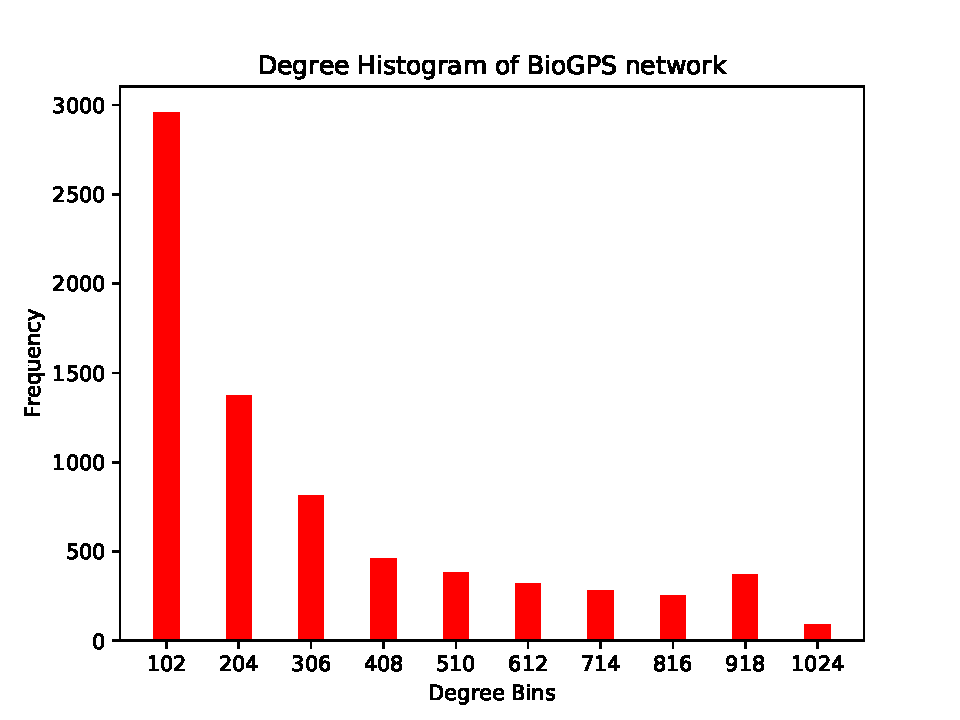
\includegraphics[width=0.5\textwidth]{degree_histogram_biogps.pdf}
\label{fig:subfig1}}
\subfloat[Subfigure 3 list of figures text][]{
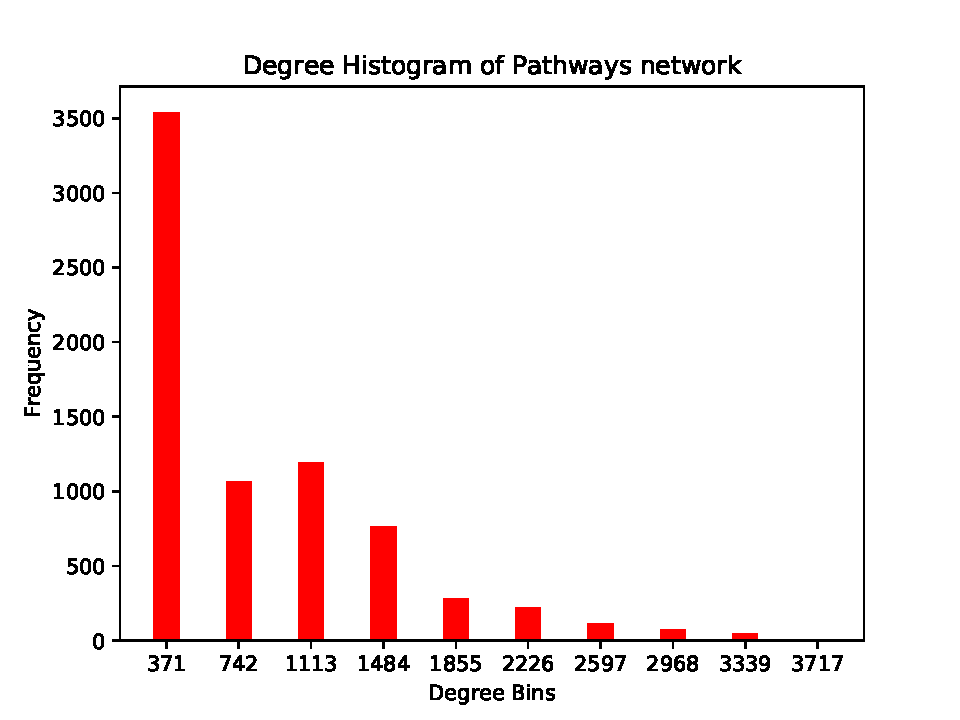
\includegraphics[width=0.5\textwidth]{degree_histogram_pathways.pdf}
\label{fig:subfig2}}
\caption{\label{fig:histograms} Outdegree distribution for nodes in the BioGPS network (a), and the Pathways network (b). The number associated to the bin is the threshold value used for the outdegree.}
\end{figure}


We followed the experimental procedure described in \cite{chen2014disease}, where $12$ diseases \cite{goh2007human} are used. Each disease is associated to at least 30 positive genes. See Table~\ref{tab:diseases} for the list of genetic diseases and the number of positive genes in each disease. For each disease, we construct a positive set $\mathcal{P}$ with all positive (confirmed) disease genes, and a negative set $\mathcal{N}$ which contains random genes associated at least to one disease class which is not related to the class that is defining the positive set. In \cite{chen2014disease} the ratio between the dataset sizes is chosen as $\vert \mathcal{N} \vert = \frac{1}{2} \vert \mathcal{P} \vert$. This is due to the fact that genes known to be related to at least one genetic disease, but not to the considered one, are well studied, so they have a low probability of being associated to the current disease.

%{\renewcommand{\arraystretch}{1.3}
%\vspace{-1.5cm}
\begin{table}
%\vspace*{1cm}
\small
\centering
\caption{\label{tab:diseases} Indices and gene number of genetic disease-gene associations.} \vspace{1em}
\label{tab:cdnk-diseases}
\setlength{\tabcolsep}{1cm}
\begin{tabular}{ccc}
\hline
Index & Disease & Number\\
\hline
0 & Connective & 35 \\
1 & Cardiovascular & 75 \\
2 & Dermatological & 54 \\
3 & Developmental & 37 \\
4 & Endocrine & 62 \\
5 & Hematological & 106 \\
6 & Immunological & 94 \\
7 & Metabolic & 159 \\
8 & Muscular & 55 \\
9 & Ophthalmological & 61 \\
10 & Renal & 42 \\
11 & Skeletal & 35 \\
\hline
\end{tabular}
\end{table}%}

In order to compare the performance of different graph node kernels, i.e. LEDK, MEDK, MDK, RLK, and CDNK., the learning algorithm is fixed. 
The predictive performance of the system using each kernel is evaluated via a leave-one-out cross validation: one gene is kept out in turn and the rest are used to train an SVM model. 
We computed a decision score $q_i$ for the test gene $g_i$ as the top percentage value of score $s_i$ among all candidate gene scores, i.e. $q_i = \frac{ |\lbrace g_j | s_i \geq s_j\rbrace |}{N}$ where $N$ is the number of candidate genes. We collected all decision scores for every gene in the test set to form a global decision score list on which we computed the AUC-ROC.

\subsection{Node Labeling} 
\label{sec:lab}
The proposed graph node kernel is able to exploit labels attached to nodes.  Labels can be discrete and/or real valued vectors. Here we discuss how to define these labels for the graphs derived from BioGPS and Pathways in such a way to enrich the amount of information that the kernel can exploit to perform its task.
Notice that the definition of the kernel allows the user to define and use any node labeling function, not only the ones we describe in the following.

\textit{Discrete labels:} we designed two different approaches to associate genes with discrete labels.

A first baseline approach is to use the same label for every node of the graph. In this case, the underpinning information for the computation of the kernel is just the topology of the neighborhood subgraphs. Topology is the information that is used by the diffusion-based kernels. Thus, this choice allows us to test whether putting the focus of attention on local topological information, as encoded by the proposed kernel, is useful or not.

The second approach aims to encode abstract information about genes into the labels. The idea, in this case, is to allow  downstream machine learning algorithms to generalize from similar examples and to allow the identification of overlooked but related genes. To this aim, we employ a gene ontology (GO) \cite{gene2004gene} to construct binary vectors representing a bag-of-terms encoding for each gene, i.e. an element of the binary vector is equal to 1 if its corresponding GO-term is associated to the gene, and is equal to 0 otherwise. The resulting vectors are then clustered using the k-means algorithm into a user defined number of classes, $P$, so that genes with similar description profiles receive the same class identifier as label.

\textit{Real vector labels:} In addition to encoding the functional information as a discrete label, we add a richer description by computing the similarity vector w.r.t. to each cluster. In this way, we can fully exploit the latent description of the genes in terms of the different functional groups captured by the clustering procedure. Formally, given a vector $v \in \mathbb{R}^{M}$ \footnote{M is the number of GO-terms, M = 26,501} we compute a similarity vector $S(v)= {s_1, s_2, \ldots, s_P}$ with entries $s_i = \frac{1}{1+ \ell(v,c_i)}$ where $\ell(v,c_i)$ is the Euclidean distance of $v$ from the center of the $i^{th}$ cluster $c_i = \frac{1}{|C_i|}\sum_{x \in C_i} x$ computed as the geometric mean of the elements in the cluster $C_i$.

\subsection{Model Selection}
The hyper-parameters of the various methods were tuned using a 10-fold cross validation. However, due to the non i.i.d. nature of the problem, we emploied a stronger setup to ensure no information leakage. The dataset $0$ (Connective) on which we  validated the performance was never subsequently used in the predictive performance estimation. The values for the diffusion parameter $\beta$ in LEDK and MEDK were sampled in $\lbrace 10^{-3}, 10^{-3}, 10^{-2}, 10^{-1} \rbrace$, time steps $t$ in MDK in $\lbrace 1, 10, 100 \rbrace$ and RLK parameter $\beta$ in $\lbrace 1, 4, 7 \rbrace$. For CDNK, the degree threshold values, $D$, were sampled in $\lbrace 10,\ 15,\ 20 \rbrace$, clique size threshold, $C$, in $\lbrace 4,\ 5 \rbrace$, maximum radius, $r^*$, in $\lbrace 1,\ 2 \rbrace$, maximum distance, $d^*$, in $\lbrace 1, 2,\ 3,\ 4 \rbrace$, number of clusters $P$ in $\lbrace 5,\ 7 \rbrace$. Finally, the regularization trade off parameter in the SVM was sampled in $\lbrace 10^{-5},  \ 10^{-4}, \ 10^{-3},\ 10^{-2},\ 10^{-1}, 1,\ 10,\ 10^2 \rbrace$. The optimal parameter values of CDNK obtained by validation process are $D = 1$, $C=5$, $r^*=2$, $d^*=1$, $P=15$ and the trade-off parameter of SVM is $10^{-2}$.
%\subsection{Parameter Impact}
%In order to evaluate the stability of kernel w.r.t the change of each parameter values, we perform experiments with disease-gene association 2 on the BioGPS network. For each parameter, first we fix the values of all other parameters, but allow the value of considered papameter to be changed. More precisely, we use the optimal tuple $C = 5,\ d^* = 1,\ D = 20,\ P = 15$ for the fixed of parameters' values. We let the changes of $C$ in $\lbrace 4,\ 5,\ 6,\ 7,\ 8,\ 9\rbrace$, $d^*$ in $\lbrace 1,\ 2,\ 3,\ 4\rbrace$, $D$ in $\lbrace 8,\ 10,\  15,\ 20,\ 30,\ 40,\ 50\rbrace$ and real vector size, $P$ in $\lbrace 8,\ 10,\ 15,\ 20,\ 30,\ 50,\ 70, 90\rbrace$.

\subsection{Results and Discussion}
%==================================================
%==================================================
%==================================================
\begin{table}[h]
\caption{Predictive performance on 11 gene-disease associations in percentage using network induced by the BioGPS. Best results in bold. We report the AUC ROC and after the ``/'' the rank for each kernel method (DK = LEDK; MD = MDK; MED = MEDK; RL = RLK; CDNK1 = ontology for discrete labels; CDNK2 = ontology for both discrete and vector labels; CDNK3 = uniform discrete labels;  CDNK4 = uniform discrete labels and ontology for vector labels.) The last two rows report the averages of AUC ROC and rank over the $11$ diseases.} \vspace{1em}
%\vspace*{5pt}
\centering
\setlength{\tabcolsep}{1mm}
\begin{tabular}{|c|c|c|c|c|c|c|c|c|}
\hline
         & \multicolumn{8}{c|}{\textbf{BioGPS}}\\
 \hline
Disease & DK & MD & MED & RL & CDNK1 & CDNK2 & CDNK3 & CDNK4\\

 \hline
1 & 51.9/8 & 57.4/7 & 59.0/6 & 59.2/5 & 65.1/4 & 69.5/3 & 72.0/2 & \textbf{72.3/1} \\

2 & 81.7/5 & 78.5/6 & 75.2/7 & 75.0/8 & 88.3/2 & \textbf{88.8/1} & 83.2/4 & 84.8/3 \\

3 & 64.3/6 & 59.6/8 & 71.6/3 & 71.8/2 & 65.5/5 & \textbf{72.5/1} & 61.4/7 & 67.9/4 \\

4 & 65.3/7 & 58.2/8 & 67.8/6 & 67.8/5 & 71.9/4 & \textbf{78.7/1} & 73.8/3 & 76.7/2 \\

5 & 64.0/8 & 64.1/7 & 66.5/5 & 66.2/6 & 75.9/4 & 76.2/3 & 77.8/2 & \textbf{78.2/1} \\

6 & 74.6/5 & 70.2/8 & 71.0/7 & 71.2/6 & 79.3/3 & \textbf{83.7/1} & 77.2/4 & 80.0/2 \\

7 & 73.0/5 & 66.7/7 & 75.4/3 & 75.6/2 & 68.8/6 & 73.9/4 & 66.1/8 & \textbf{77.4/1} \\

8 & 74.4/8 & 76.8/3 & 76.2/5 & 76.4/4 & 74.7/7 & 77.7/1 & 76.1/6 & 76.9/2 \\

9 & 71.5/2 & 65.6/8 & 67.7/6 & 69.9/3 & 66.8/7 & \textbf{71.7/1} & 67.9/5 & 68.1/4 \\

10 & 54.0/6 & 50.3/8 & 56.1/5 & 51.1/7 & 77.6/4 & \textbf{82.7/1} & 77.7/3 & 78.3/2 \\

11 & 58.2/7 & 51.3/8 & 59.3/6 & 59.3/5 & 71.8/4 & \textbf{80.2/1} & 74.8/2 & 74.0/3 \\

\hline
$\overline{AUC}$ & 66.6	& 63.5 & 67.8 &	67.6 & 73.2 & \textbf{77.8} & 73.5 & 75.9 \\


$\overline{Rank}$ & 6.09 & 7.09 &  5.36 & 4.82 & 4.45 & \textbf{1.64} & 4.18 & 2.27 \\
 \hline 
\end{tabular}
\label{tab:cdnk-biogps}
\end{table}
%=====================================
%=====================================
\begin{table}[h]
\caption{Predictive performance on 11 gene-disease associations in percentage using network induced by the Pathways. Best results in bold. We report the AUC ROC and after the ``/'' the rank for each kernel method (DK = LEDK; MD = MDK; MED = MEDK; RL = RLK; CDNK1 = ontology for discrete labels; CDNK2 = ontology for both discrete and vector labels; CDNK3 = uniform discrete labels;  CDNK4 = uniform discrete labels and ontology for vector labels.) The last two rows report the averages of AUC ROC and rank over the $11$ diseases.} \vspace{1em}
%\vspace*{5pt}
\centering
\setlength{\tabcolsep}{1mm}
\begin{tabular}{|c|c|c|c|c|c|c|c|c|}
\hline
         & \multicolumn{8}{c|}{\textbf{Pathways}} \\
 \hline
Disease & DK & MD & MED & RL & CDNK1 & CDNK2 & CDNK3 & CDNK4 \\

 \hline
1 & 74.7/8 & 76.4/7 & 78.7/6 & 78.8/5 & 80.2/4 & 82.4/2 & \textbf{82.8/1} & 82.3/3 \\

2 & 55.1/8 & 64.9/7 & 76.6/6 & 76.6/5 & 81.1/2 & 80.3/4 & 80.1/3 & \textbf{81.9/1} \\

3 & 55.0/8 & 62.7/7 & 64.1/5 & 65.6/4 & 67.1/3 & 63.6/6 & 69.7/2 & \textbf{71.4/1} \\

4 & 54.3/8 & 65.2/6 & \textbf{73.7/1} & 73.7/2 & 66.1/5 & 68.1/3 & 64.0/7 & 67.3/4 \\

5 & 52.9/8 & 55.7/7 & 62.7/5 & 62.7/6 & 68.3/2 & \textbf{69.6/1} & 66.2/4 & 68.1/3 \\

6 & 83.4/8 & 92.7/7 & 96.5/2 & \textbf{96.5/1} & 93.0/6 & 94.1/5 & 94.5/4 & 94.9/3 \\

7 & 84.5/7 & 88.3/8 & 89.4/2 & \textbf{89.5/1} & 88.5/6 & 88.5/5 & 89.0/3 & 88.7/4 \\

8 & 53.7/8 & 65.6/7 & 72.0/6 & 72.3/5 & 72.5/4 & 72.5/3 & 74.9/2 & \textbf{75.3/1} \\

9 & 52.5/8 & 64.9/5 & 64.2/7 & 64.2/6 & \textbf{81.3/1} & 81.0/3 & 80.1/2 & 79.8/4 \\

10 & 68.8/6 & 65.4/8 & 74.4/5 & 74.4/4 & 66.9/7 & 76.8/2 & 75.2/3 & \textbf{78.7/1} \\

11 & 53.7/8 & 69.2/7 & 74.6/5 & 74.1/6 & 77.0/3 & \textbf{78.7/1} & 75.1/4 & 77.3/2 \\

\hline
$\overline{AUC}$ & 62.6	& 70.1 & 75.2 & 75.3 & 76.5 & 77.8 & 77.4 &	\textbf{78.7}
 \\
$\overline{Rank}$ & 7.73 & 6.82 & 4.55 & 4.09 & 3.91 & \textbf{2.27} & 3.18 & 2.45 \\
 \hline 
\end{tabular}
\label{tab:cdnk-pathways}
\end{table}
Tables \ref{tab:cdnk-biogps} and \ref{tab:cdnk-pathways} report the AUC-ROC performance of the different diffusion-based graph node kernels and the different variations of CDNK on BioGPS and Pathways networks, respectively. In what follows, we analyze the results to answer to the two research questions we posed at the beginning of the section.

Concerning {\it Q1}, i.e. improvement on the performance of diffusion-based graph node kernels, CDNK variations outperformed diffusion-based graph node kernels in almost all cases on BioGPS network. For the moment, we postpone the discuss of these cases. When looking at the Pathways network, CDNK variations were outperformed by one of the diffusion-based graph node kernels in only $3$ out of $11$ cases. 
When looking at the average results, it is clear that
CDNK variations are ranked first when considering both the average AUC-ROC and the average rank with a difference, w.r.t. the best diffusion-based kernel, ranging from $5.4\%$ to $10\%$ and from $1.2\%$ to $3.4\%$ on BioGPS and Pathways, respectively. As a consequence, we can conclude that CDNK variations show state-of-the art performance in graph node kernels for this task. Thus, the answer to question {\it Q1} is positive.

Let now turn our attention to question {\it Q2}, i.e. whether the possibility to use local topology and/or real valued information is useful to improve performance.
The first part of the question, i.e. usefulness of local topology, can be answered by looking at results of CDNK3, where only discrete labels defined by the baseline approach are used. If we look at results obtained on BioGPS network, we see that CDNK3 outperforms diffusion-based kernels with the 
 exceptions of datasets $3$, $7$, $8$, and $9$, thus $7$ times over $11$. It is important to stress, however, that on the average CDNK3 outperformed the diffusion-based kernels of $10.19\%$, while it was outperformed on the average of $6.05\%$. An even better scenario is observed for the Pathways network, where only in one case (dataset $4$) the performance of CDNK3 was inferior of almost all diffusion-based kernels.
Thus, it seems that exploiting local topological information is actually important in many cases. 
Regarding the integration of real valued vectors, we have to look at variations CDNK2 and CDNK4, that exploit real valued labels based on GO.
It is readily evident that CDNK2 and CDNK4 improve on the performance of diffusion-based kernels in most cases. Specifically, for BioGPS network,
CDNK2 is the best performer in absolute in $7$ out of $11$ datasets. Moreover, its worst performance places it above all diffusion-based kernels.
In turn, CDNK4 is first in $3$ datasets and second in $4$ datasets, and again its worst performance places it above all diffusion-based kernels.
When looking at the results for the Pathways network, CDNK4 is the best performer among all kernels, while CNDK2 places in second position since
even if it is first on two datasets as well as RLK, RLK has a worst ranking score on most of the other datasets.
We can conclude that also the exploitation of real valued information seems to improve the performance. Thus, also for question  {\it Q2} we can give a positive answer.
%In particular, considering the use of discrete labels based on ontology, using side information helps to increase the performance in all diseases on BioGPS and in 9 out of 11 diseases on Pathways. Similarly, by employing auxiliary information associated to graph nodes, the performance of CNDK in case of using uniform discrete labels is also improved in 9 and 8 out of 11 on BioGPS and Pathways, respectively.

\subsection{Sensitivity Analysis for Hyper-parameters}
In order to support our claims in Section~\ref{hyper}, we performed the following experiment with kernel CDNK4. For the BioGPS network we selected disease 2 (Dermatological)
and, starting from the configuration of the values for the hyper-parameters selected by the model selection procedure, we in turn moved the value of each hyper-parameter, monitoring the change in performance. We left unchanged the maximum radius ($r^*$) for computational reasons: having too big neighborhood subgraphs makes computation of isomorphism too heavy and significantly reduces the likelihood of finding matchings. The obtained results are shown in Figure~\ref{fig:globfig}.
It can be observed that the range of values where the performance is maximal is located around small values for the hyper-parameters, thus confirming that too low or too high values for the hyper-parameters do not bring good performances.

%==================================================
\begin{figure}[h]
\centering
\subfloat[Subfigure 2 list of figures text][]{
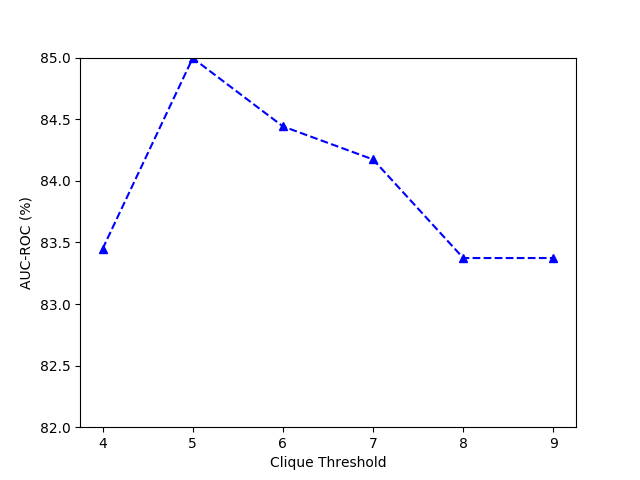
\includegraphics[width=0.4\textwidth]{cliques.png}
\label{fig:subfig1}}
\subfloat[Subfigure 3 list of figures text][]{
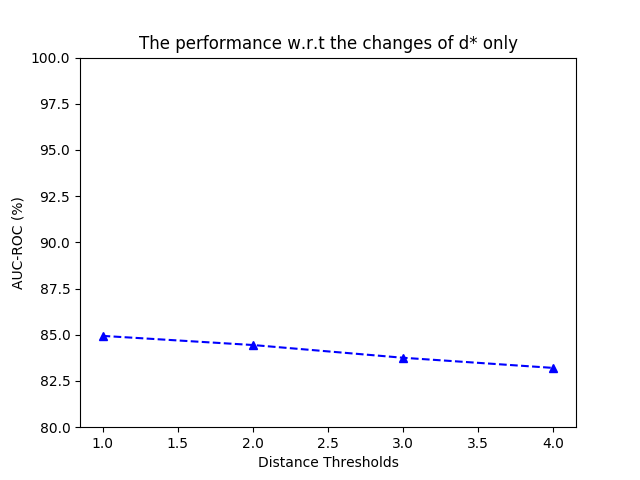
\includegraphics[width=0.4\textwidth]{distance.png}
\label{fig:subfig2}}
\qquad
\subfloat[Subfigure 2 list of figures text][]{
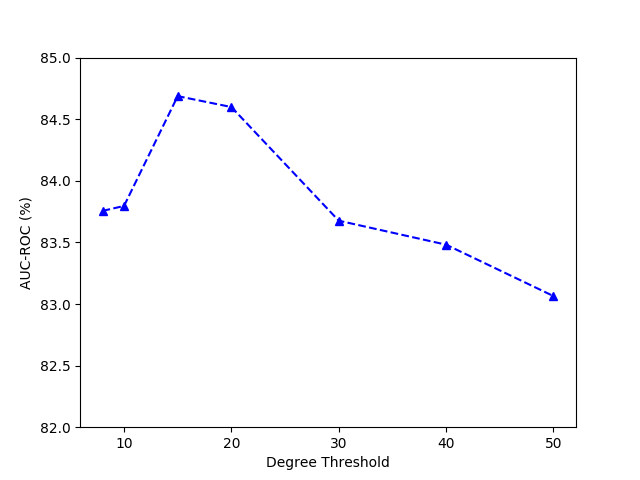
\includegraphics[width=0.4\textwidth]{degree.png}
\label{fig:subfig3}}
\subfloat[Subfigure 3 list of figures text][]{
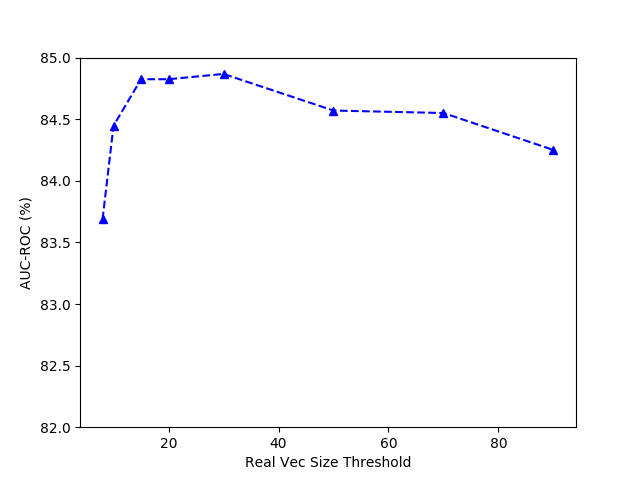
\includegraphics[width=0.4\textwidth]{vec_size.png}
\label{fig:subfig4}}
\caption{\label{fig:globfig} Performance of CDNK4 on the BioGPS network for disease 2 (Dermatological) w.r.t the change of most of the hyper-parameters: (a) clique threshold ($C$); (b) distance threshold ($d^*$); (c) degree threshold ($D$); (d) real vec size threshold ($P$). The radius ($r^*$) was not changed because of computational reasons.}
\end{figure}

\section{Conclusion and Future Work}
We have shown how decomposing a network in a set of connected sparse graphs allows us to take advantage of the discriminative power of CDNK, a novel decomposition kernel, to achieve state-of-the-art results for a disease gene prioritization task.
Moreover, we have also introduced the possibility to integrate in the kernel computation  additional information in the form of real valued vectors in the case in which it is available for graph nodes. We experimentally showed that this possibility actually leads to even better performances. Future work we will investigate on how to: \textit{i}) decompose networks in a data driven way; \textit{ii}) extend the CDNK approach to gene-disease association problems exploiting multiple heterogeneous information sources in a joint way.


\section*{Funding}
This work was supported by the University of Padova, Strategic Project BIOINFOGEN.
\section*{References}

\bibliography{mybibfile}
\end{document}
